\chapter{Analisi dei dati e risultati}
\section{Dataset e hardware utilizzato}

Per evidenziare le capacità e le potenzialità del software sviluppato, sono state condotte diverse analisi esemplificative basate su un ampio volume di dati bibliografici. A tal fine, sono stati raccolti tutti gli articoli pubblicati nell'ambito ``Computer Science'' dal 1850 al 2022, per un totale di 8.2 milioni. Questo corpus, di dimensioni notevoli, riflette lo sviluppo storico e l'evoluzione dell'informatica. Nonostante ciò, a causa di restrizioni imposte dalle API per l'accesso ai dati, sono state raccolte informazioni complete su soli circa 460.000 autori, una porzione significativa, ma non completa, dei 6.6 milioni di autori totali in questo campo. Un riassunto dettagliato del dataset è presentato nella Tabella~\ref{tab:overview_dataset}.
Questo insieme di dati, sebbene non totalmente rappresentativo dell'intera comunità accademica in informatica, fornisce un quadro chiaro delle tendenze e delle evoluzioni tecnologiche che hanno segnato quasi due secoli di ricerca.

\begin{table}[ht]
    \centering
    \begin{tabular}{|l|r|r|}
        \hline
        \textbf{Collezione} & \textbf{Documenti}  & \textbf{Dimensione totale} \\
        \hline
        \texttt{collectionAuthors} & $466\cdot10^3$ su $6.6\cdot10^6$ &  5.15 GiB \\
        \hline
        \texttt{collectionAbstracts} & $8.2\cdot10^6$ & 17.47 GiB \\
        \hline
        \texttt{collectionAuthorsAggregate} & $466\cdot10^3$ & 17.66 GiB \\
        \hline
    \end{tabular}
    \caption{Panoramica dati scaricati per analisi}
    \label{tab:overview_dataset}
\end{table}

Le analisi sono state effettuate su un MacBook Pro equipaggiato con un chip M1 Pro e 16 GiB di memoria RAM, operante con il sistema operativo macOS versione 13.6 (22G120). Il processo analitico è stato gestito attraverso un ambiente Docker (v24.0.6), ottimizzato per sfruttare al meglio le risorse hardware disponibili. In particolare, il container Docker è stato configurato per utilizzare tutti i 10 core del dispositivo, allocando alla macchina virtuale 12 GiB di RAM e 3 GiB di memoria swap aggiuntiva.

\section{Analisi e grafici}
Al fine di testare approfonditamente il software sviluppato, è stata pianificata l'esecuzione di quattro diverse analisi, ciascuna con soglie distinte di $h$-index: 50, 100, 150 e 200. L'obiettivo di questa sperimentazione era duplice: in primo luogo, valutare il tempo di risposta del software in seguito alla chiamata dell'API, e in secondo luogo, analizzare le dimensioni del documento JSON fornito in risposta. Queste metriche sono cruciali per determinare sia l'efficienza operativa del software sia la sua capacità di gestire richieste di dati di varie grandezze. I risultati di queste analisi, che riflettono l'efficacia del software sotto diverse condizioni operative, sono riportati nella Tabella~\ref{tab:overview_metrics_performance}. Questi dati forniscono un'importante indicazione sulle prestazioni e l'affidabilità del sistema in scenari di utilizzo reali, offrendo un quadro chiaro dell'adattabilità e della robustezza del software.

\begin{table}[ht]
    \centering
    \begin{tabular}{|r|r|r|}
        \hline
        \textbf{$h$-index minimo} & \textbf{Tempo di risposta} & \textbf{Dimensione} \\
        \hline
        50 & 6.5 min & 2.1 MiB \\
        \hline
        100 & 4.8 min & 1.6 MiB \\
        \hline
        150 & 4.5 min & 1.5 MiB \\
        \hline
        200 & 4.7 min & 1.5 MiB \\
        \hline
    \end{tabular}
    \caption{Metriche di performance delle analisi}
    \label{tab:overview_metrics_performance}
\end{table}

Per il presente studio, sono stati selezionati i grafici relativi alle analisi con soglie di $h$-index pari a 50 e 150, considerate le più significative.

\begin{figure}[ht]
    \centering
    \begin{subfigure}{0.49\textwidth}
        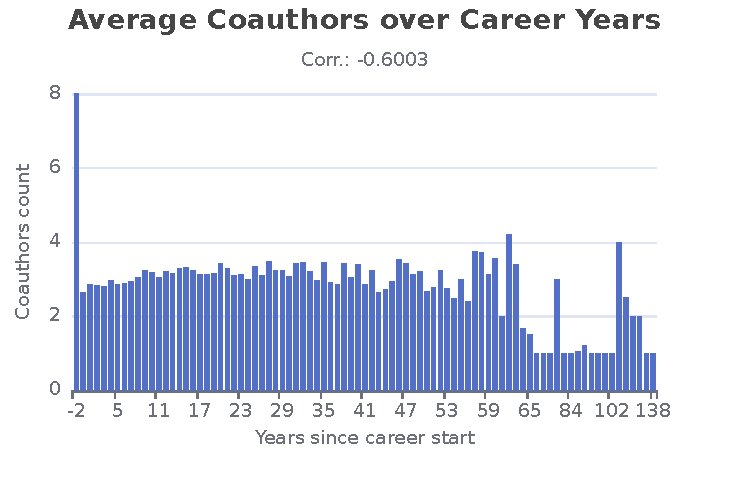
\includegraphics[width=\textwidth]{images/Average-Coauthors-over-Career-Years-50.pdf}
        \caption{Soglia 50}
        \label{fig:Average-Coauthors-over-Career-Years-50}
    \end{subfigure}
    \hfill
    \begin{subfigure}{0.49\textwidth}
        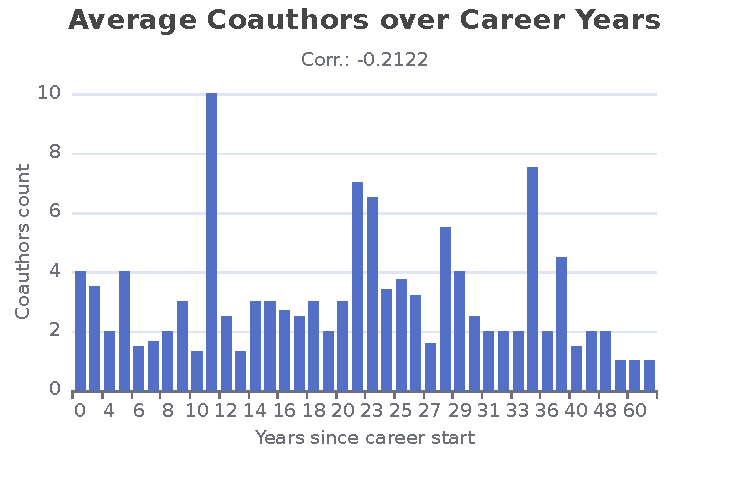
\includegraphics[width=\textwidth]{images/Average-Coauthors-over-Career-Years-150.pdf}
        \caption{Soglia 150}
        \label{fig:Average-Coauthors-over-Career-Years-150}
    \end{subfigure}        
    \caption{Grafici della variazione media dei coautori nel tempo}
    \label{fig:Average-Coauthors-over-Career-Years}
\end{figure}

Il confronto visualizzato in Figura~\ref{fig:Average-Coauthors-over-Career-Years} illustra l'evoluzione delle dinamiche di collaborazione tra i ricercatori nel corso della loro carriera. Dall'analisi emerge una tendenza generale alla riduzione del numero di coautori nel tempo. Interessante notare come questa tendenza sia meno marcata negli autori con un $h$-index più elevato, suggerendo che i ricercatori più affermati mantengano un livello di collaborazione più costante rispetto ai loro colleghi.

\begin{figure}[ht]
    \centering
    \begin{subfigure}{0.49\textwidth}
        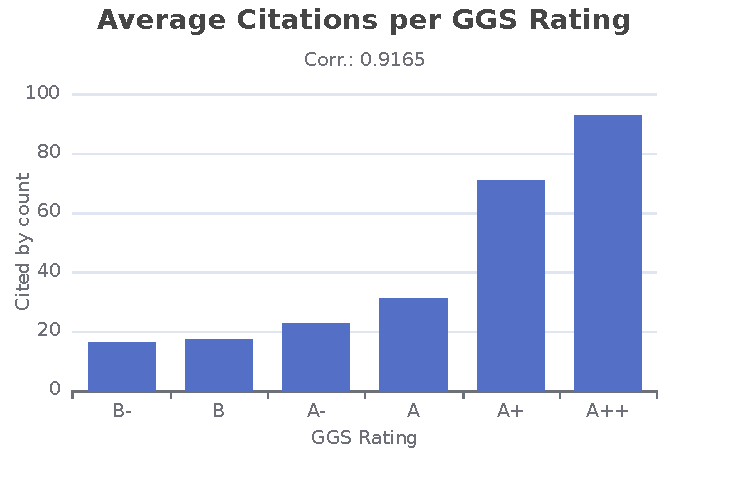
\includegraphics[width=\textwidth]{images/Average-Citations-per-GGS-Rating-50.pdf}
        \caption{Soglia 50}
        \label{fig:Average-Citations-per-GGS-Rating-50}
    \end{subfigure}
    \hfill
    \begin{subfigure}{0.49\textwidth}
        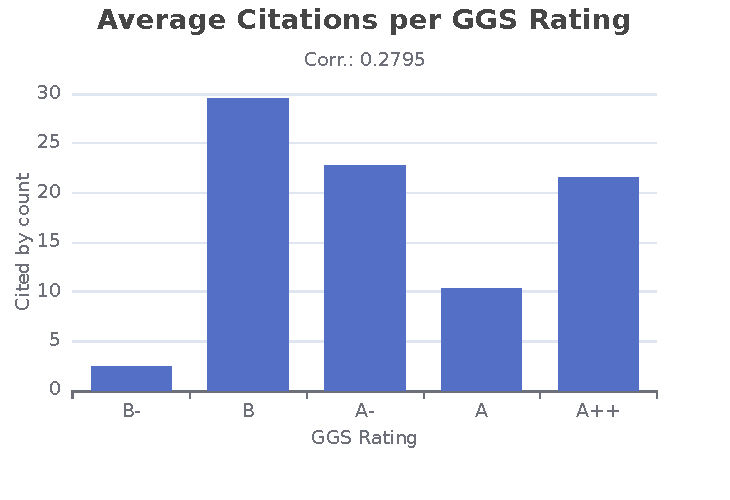
\includegraphics[width=\textwidth]{images/Average-Citations-per-GGS-Rating-150.pdf}
        \caption{Soglia 150}
        \label{fig:Average-Citations-per-GGS-Rating-150}
    \end{subfigure}        
    \caption{Grafici dell'impatto del rating di una conferenza sul numero di citazioni}
    \label{fig:Average-Citations-per-GGS-Rating}
\end{figure}

La Figura~\ref{fig:Average-Citations-per-GGS-Rating} illustra la relazione tra la classificazione delle conferenze informatiche e il numero medio di citazioni per articolo. È evidente che, per il gruppo con un $h$-index superiore a 50, esiste una forte relazione tra il prestigio del convegno e il numero di citazioni ricevute. Tuttavia, interessante notare come l'influenza della reputazione del congresso tenda a diminuire all'aumentare della soglia dell'$h$-index. Questo fenomeno suggerisce che, per gli autori con un elevato impatto nel mondo accademico, altri fattori oltre alla semplice reputazione del convegno possono avere un maggiore impatto sulle citazioni ricevute dai loro articoli.

\begin{figure}[ht]
    \centering
    \begin{subfigure}{0.49\textwidth}
        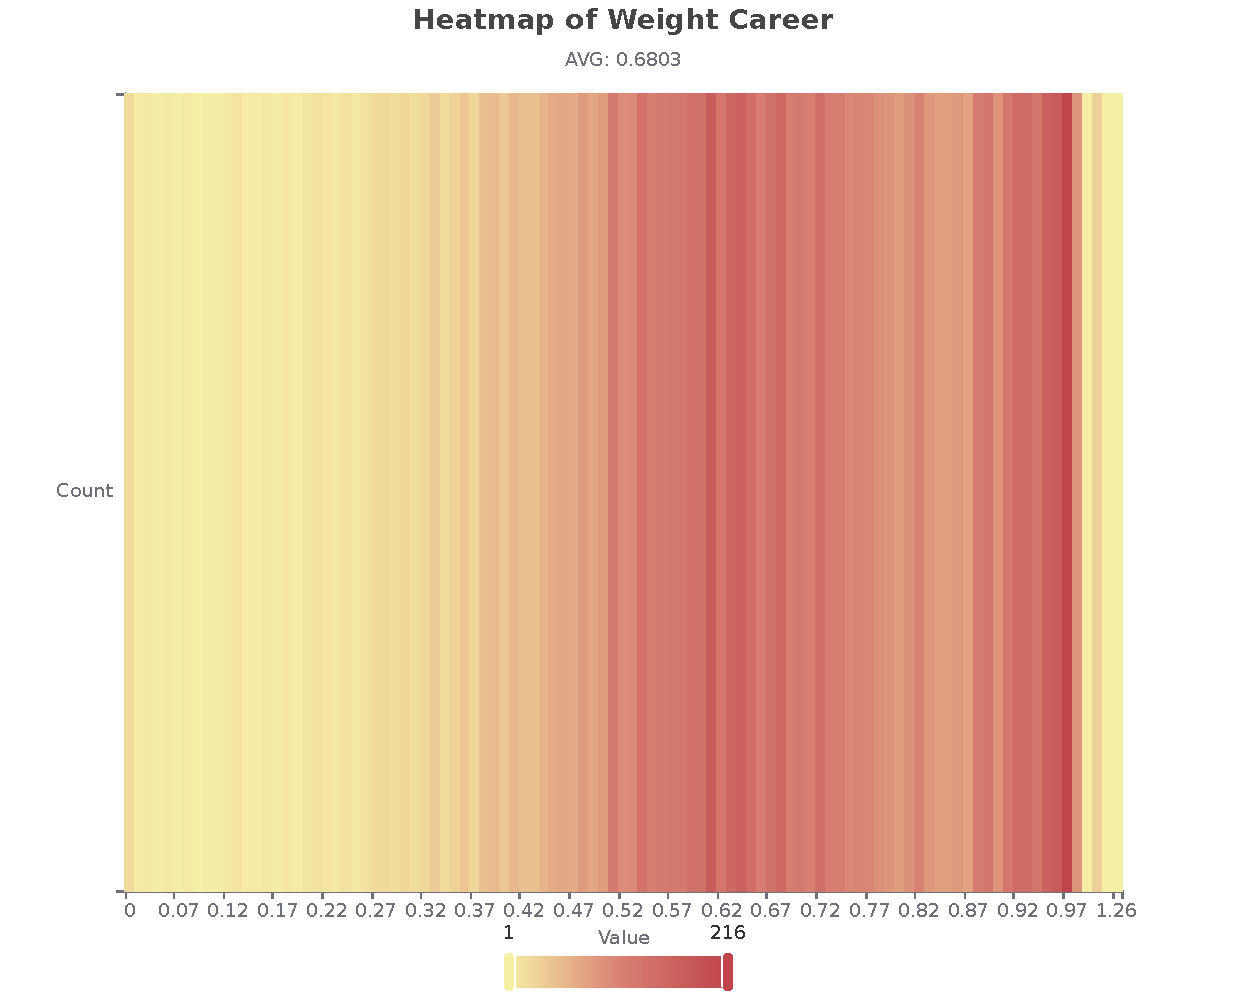
\includegraphics[width=\textwidth]{images/Heatmap-of-Weight-Career-50.pdf}
        \caption{Soglia 50}
        \label{fig:Heatmap-of-Weight-Career-50}
    \end{subfigure}
    \hfill
    \begin{subfigure}{0.49\textwidth}
        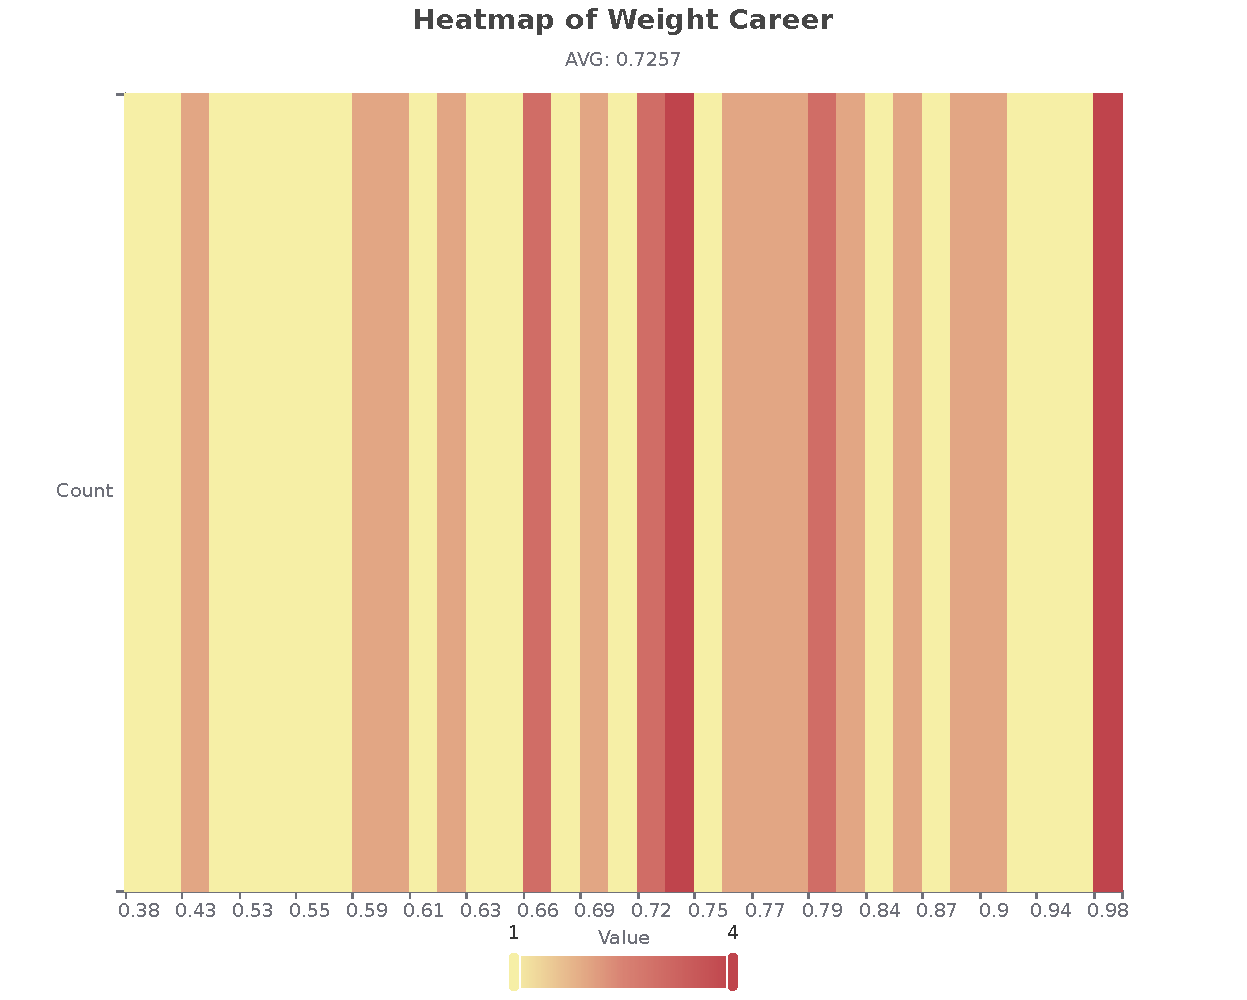
\includegraphics[width=\textwidth]{images/Heatmap-of-Weight-Career-150.pdf}
        \caption{Soglia 150}
        \label{fig:Heatmap-of-Weight-Career-150}
    \end{subfigure}        
    \caption{Grafici dell'analisi del momento di pubblicazione di articoli influenti sull'$h$-index}
    \label{fig:Heatmap-of-Weight-Career}
\end{figure}

L'analisi visualizzata nella Figura~\ref{fig:Heatmap-of-Weight-Career} mette in luce un aspetto relativo alla carriera accademica degli autori: in media, gli articoli che influenzano maggiormente l'$h$-index tendono a essere pubblicati dopo la metà della loro carriera, questa tendenza si mantiene con un impatto maggiore per tutta la seconda metà della loro attività accademica, suggerendo che il periodo più produttivo e influente per molti ricercatori si verifica nella fase matura della loro carriera.

\begin{figure}[ht]
    \centering
    \begin{subfigure}{0.49\textwidth}
        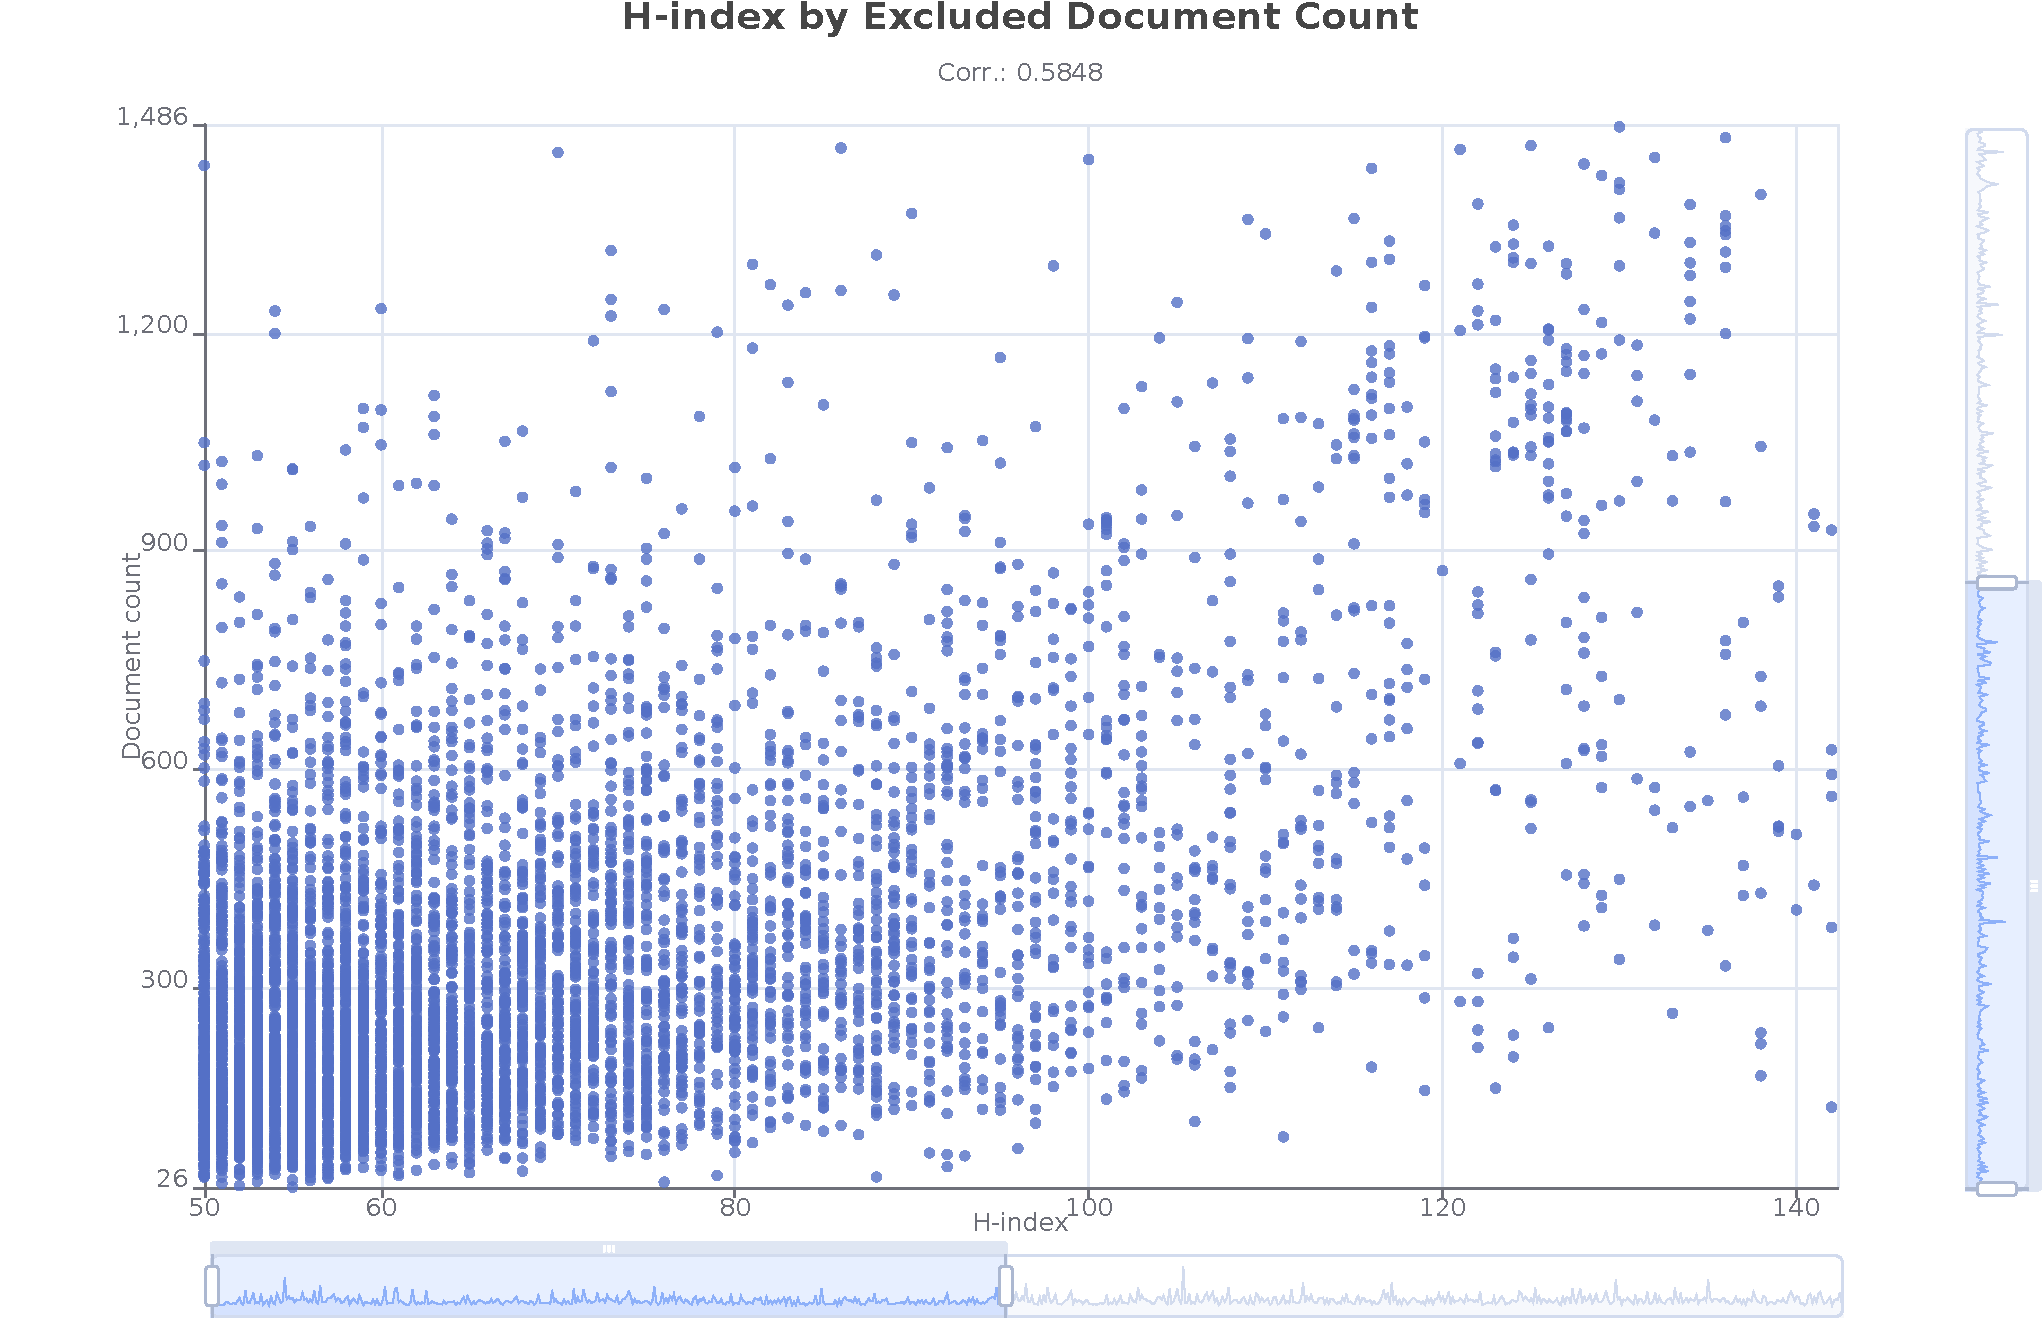
\includegraphics[width=\textwidth]{images/H-index-by-Excluded-Document-Count-50.pdf}
        \caption{Soglia 50}
        \label{fig:H-index-by-Excluded-Document-Count-50}
    \end{subfigure}
    \hfill
    \begin{subfigure}{0.49\textwidth}
        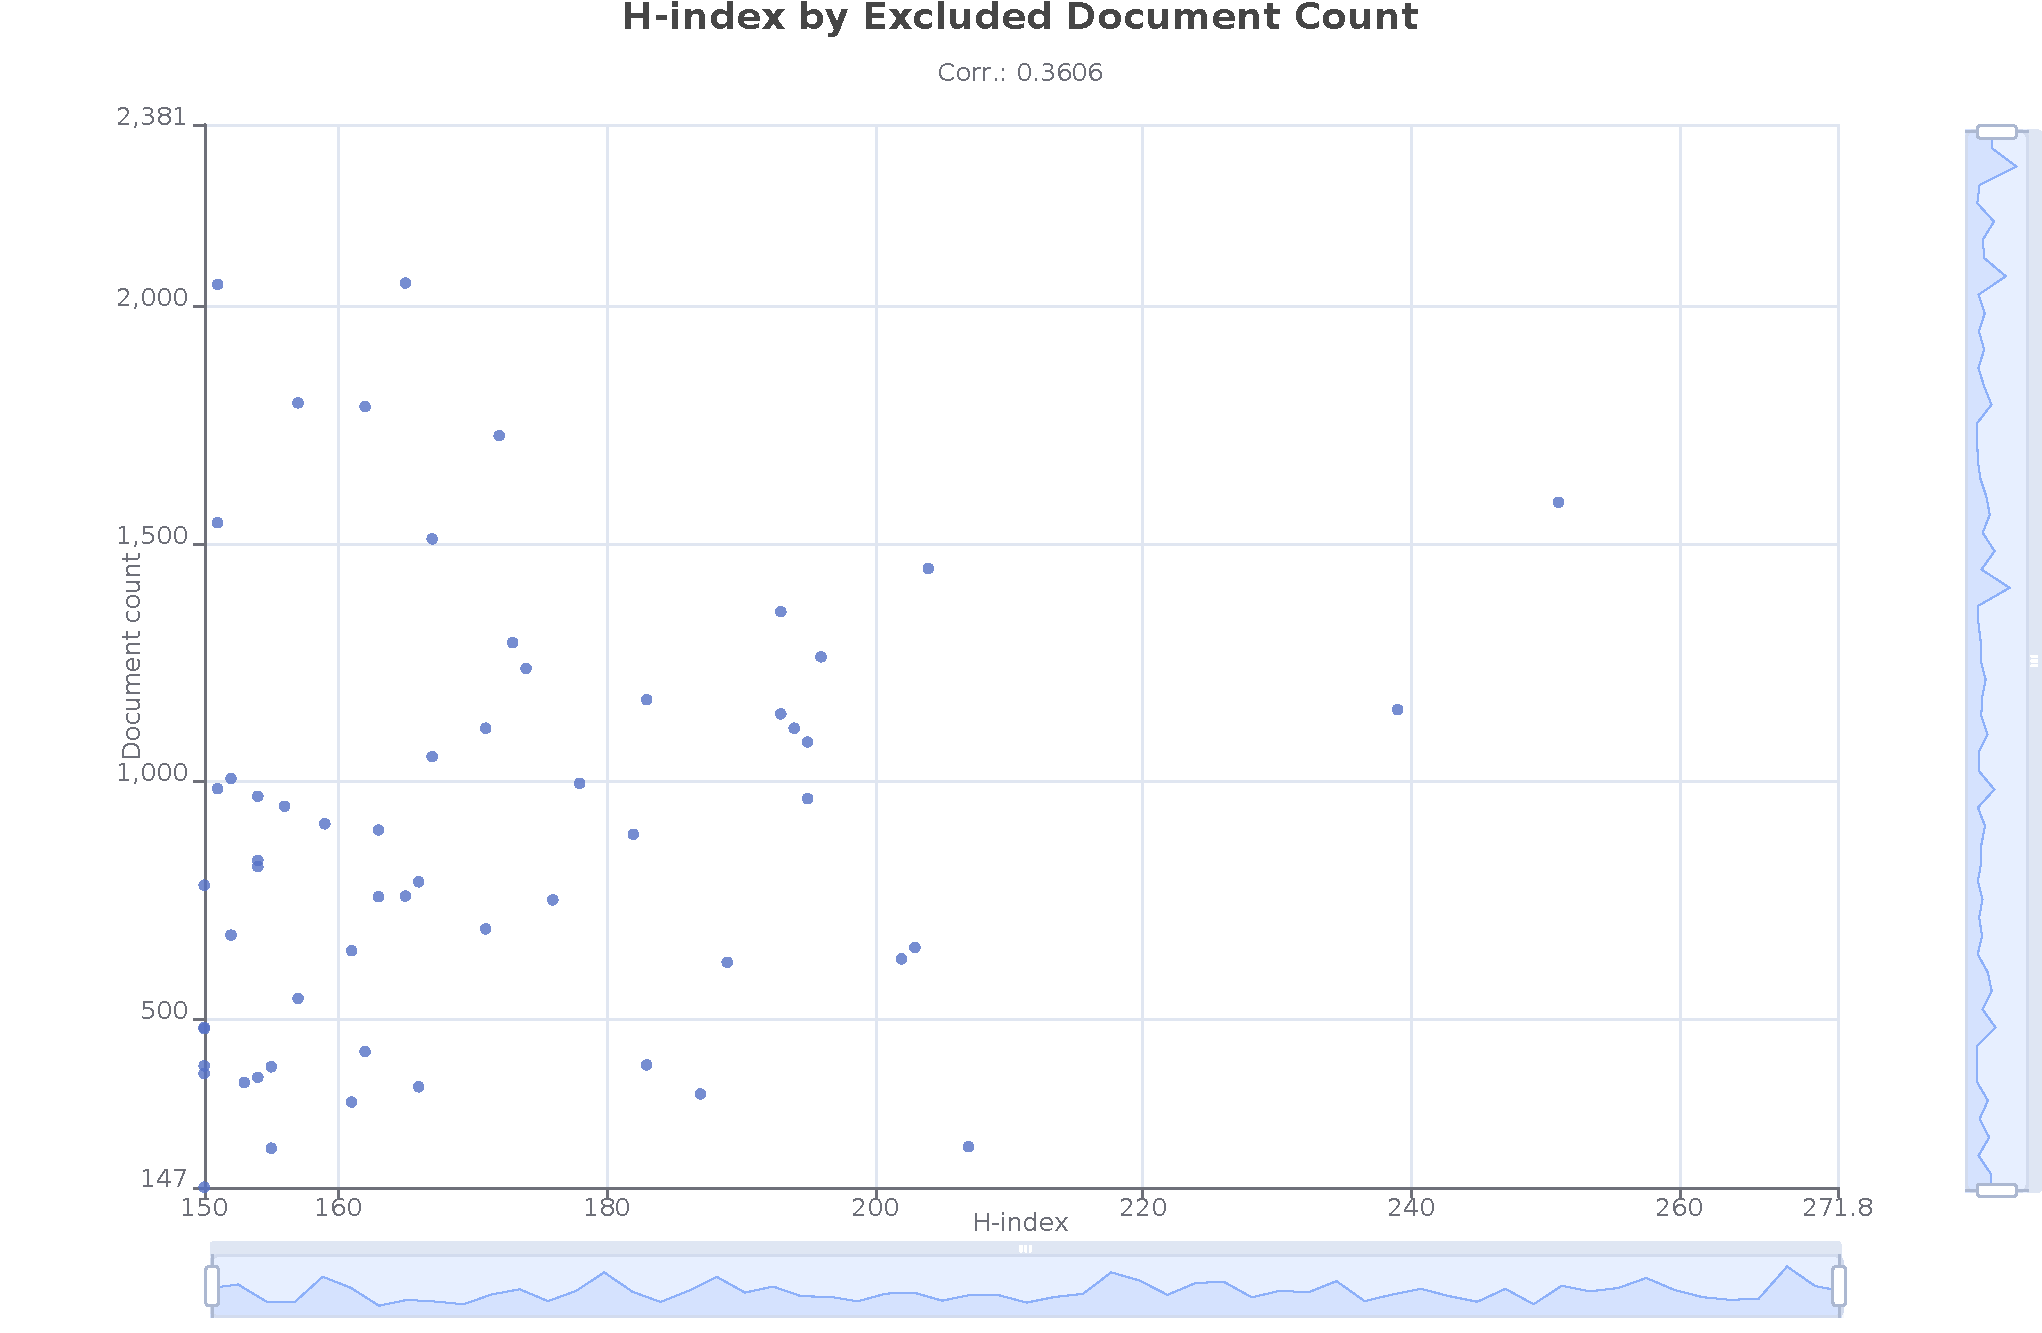
\includegraphics[width=\textwidth]{images/H-index-by-Excluded-Document-Count-150.pdf}
        \caption{Soglia 150}
        \label{fig:H-index-by-Excluded-Document-Count-150}
    \end{subfigure}        
    \caption{Grafico della correlazione tra $h$-index e articoli esclusi}
    \label{fig:H-index-by-Excluded-Document-Count}
\end{figure}

L'analisi della correlazione tra l'$h$-index degli autori e il numero di documenti esclusi dal calcolo di quest'ultimo è descritta in Figura~\ref{fig:H-index-by-Excluded-Document-Count}. Si osserva una correlazione moderata, che implica che gli autori con un numero maggiore di lavori tendono generalmente ad avere un valore più elevato. Questo suggerisce che una produttività accademica più alta può portare a un indice di impatto più alto, anche se non tutti i documenti contribuiscono direttamente all'$h$-index.

La relazione tra il conteggio degli autori di un articolo e il numero di citazioni ricevute è mostrato in Figura~\ref{fig:Citations-by-Author-Count}. Il grafico mostra una correlazione molto debole  tra queste due variabili, suggerendo che il numero di ricercatori di un paper non ha un impatto significativo sul numero di citazioni ricevute.

\begin{figure}[ht]
    \centering
    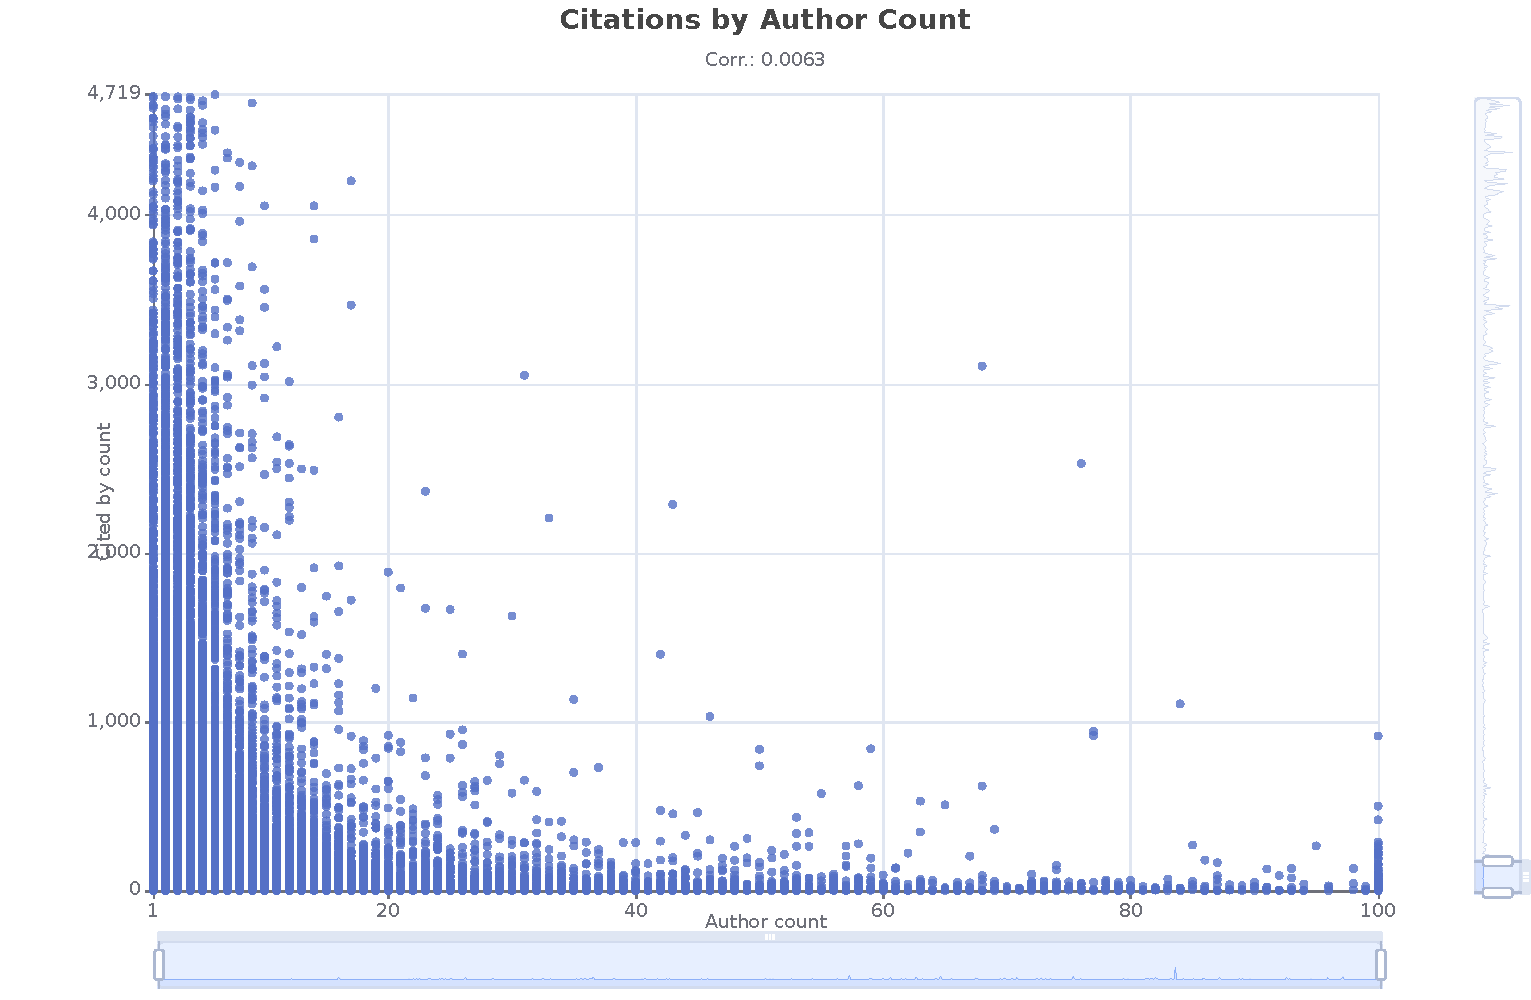
\includegraphics[width=.7\textwidth]{images/Citations-by-Author-Count.pdf}
    \caption{Grafico dell'impatto del numero di coautori sulle citazioni}
    \label{fig:Citations-by-Author-Count}
\end{figure}

La Figura~\ref{fig:H-index-by-Duration-career} evidenzia una correlazione sostanziale tra la durata della carriera di un autore e il suo $h$-index indicando che generalmente un valore più alto corrisponde a una carriera più lunga nel campo della ricerca. La relazione tra questi due fattori sottolinea l'importanza dell'esperienza e del tempo dedicato in ambito accademico nell'incrementare l'accumulo di citazioni e, di conseguenza, nell'ottenere un $h$-index elevato.

\begin{figure}[ht]
    \centering
    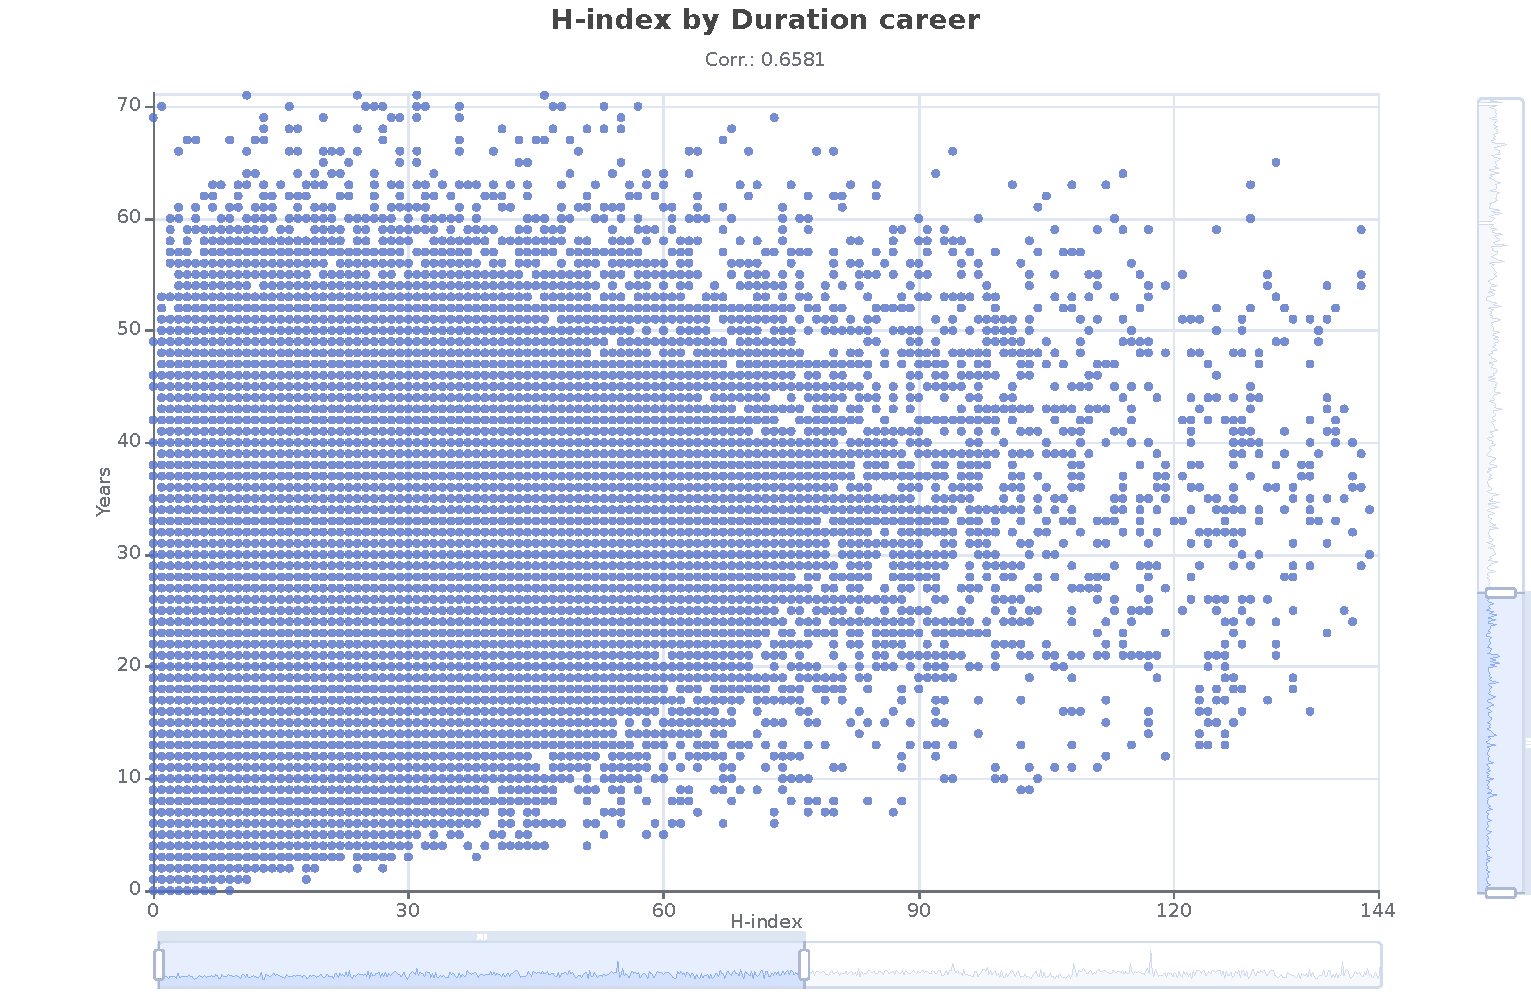
\includegraphics[width=.7\textwidth]{images/H-index-by-Duration-career.pdf}
    \caption{Correlazione tra $h$-index e durata della carriera}
    \label{fig:H-index-by-Duration-career}
\end{figure}


\section{Commenti e riflessioni sui risultati}
Esaminando nel loro insieme i risultati dei grafici, emerge un quadro complesso e dettagliato della carriera accademica, caratterizzato da dinamiche interessanti.
Questi dati rivelano che, indipendentemente dal livello di $h$-index, esistono trend comuni ma anche differenze significative nelle traiettorie accademiche. Per esempio, la tendenza alla riduzione delle collaborazioni nel corso della carriera è meno evidente negli autori con un $h$-index molto elevato. Questo suggerisce che i ricercatori più affermati, forse a causa della loro consolidata reputazione e rete di contatti, mantengono un livello di collaborazione elevato e stabile.

Inoltre, l'influenza della reputazione delle conferenze sul numero di citazioni ricevute tende a diminuire all'aumentare dell'$h$-index, ciò potrebbe indicare che, per i ricercatori di alto livello, la qualità e l'originalità della ricerca diventano più importanti del prestigio del convegno per ottenere riconoscimenti.

L'analisi sull'età dei contributi significativi per l'indice bibliometrico suggerisce che i ricercatori più esperti tendono a produrre lavori di impatto maggiore nella fase matura della loro carriera, forse grazie a una maggiore profondità di conoscenza e a reti di collaborazione ben sviluppate.

Infine, la correlazione tra la durata della carriera e l'$h$-index enfatizza l'importanza dell'esperienza prolungata e dell'impegno costante nella ricerca. I ricercatori con carriere più lunghe non solo hanno più tempo per pubblicare e accumulare citazioni, ma anche per sviluppare e affinare le loro competenze di ricerca.

In conclusione, questi grafici illustrano l'importanza di una visione a lungo termine nella carriera accademica, dove la costruzione di reti solide, la scelta strategica delle conferenze, e l'approfondimento continuo delle competenze di ricerca sono cruciali per raggiungere e mantenere un alto livello di impatto e riconoscimento nel campo accademico.